%\red{
\section{Conclusion and Future Work}
\label{subsec:disc}

%\subsection{Generalization}
%The techniques introduced via DROP can benefit any repeated-query setting where PCA is the method of choice, so long as users are willing to sacrifice small amounts of accuracy for improved running time and a metric of interest can be defined for the application (i.e., $TLB$ for similarity search, or loss function estimates for more general tasks). 
%For instance, examining a recent natural language processing application of PCA as a word vector post-processing step prior to downstream workloads~\cite{allbut} is exciting future work. 
%While having an exact runtime model is not common a priori, many common analytics workloads for clustering, classification, or regression, black-box techniques (as we used for k-NN and k-means) can be applied as downstream tasks can be performed as a series of matrix decompositions and multiplies (i.e., techniques that make use of gradient descent). 
%}
DROP provides a first step in bridging the gap between quality and efficiency in DR for downstream \red{analytics}.
However, there are several avenues to explore for future work, such as sophisticated sampling methods and streaming execution.

%We demonstrated that workload-aware approximate PCA can provide large end-to-end speedups in \red{our time series case study} and for non-time series datasets with low intrinsic dimensionality.

DROP's efficiency is determined by the dataset's spectrum; MALLAT, with the sharpest drop-off, performs extremely well, and Phoneme, with a near uniform distribution, does not.
Datasets such as Phoneme perform poorly under the default configuration as we enable cost-based optimization after reaching a feasible point.
Thus, DROP spends a disproportionate time sampling (Fig.~\ref{fig:lesion}c). 
Extending DROP to determine if a dataset is amenable to aggressive sampling is an exciting area of future work. 
For instance, recent theoretical results that use sampling to estimate spectrum, even when the number of samples is small in comparison to the input dimensionality~\cite{estspec}, can be run alongside DROP.

%To combat this, we provide an alternate sampling schedule that aggressively increases the sampling rate to quickly reach a $TLB$-achieving state if DROP repeatedly fails to meet the target $TLB$. 

%\vspace{.2cm}
%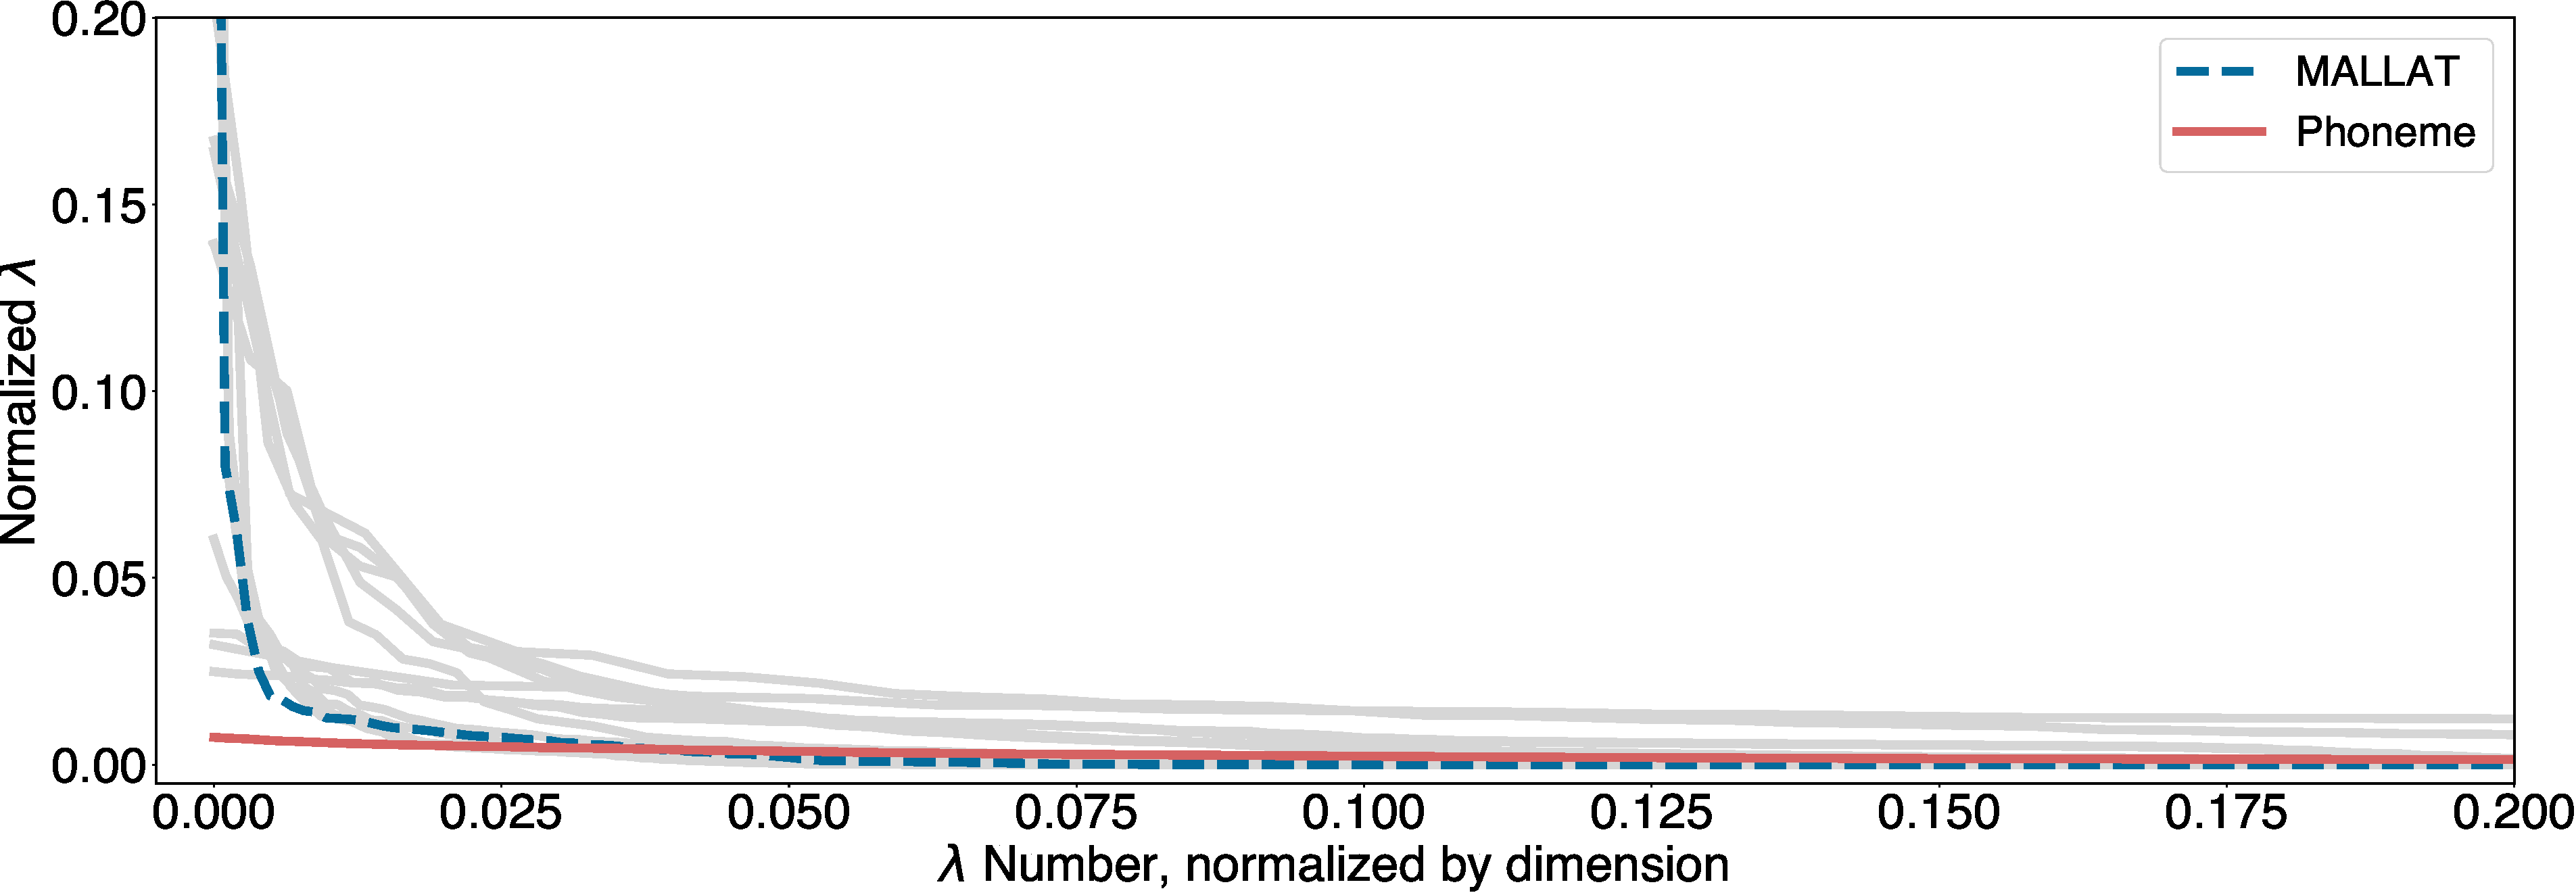
\includegraphics[width= .9\linewidth]{figs/spectrum-rev.pdf}

%\begin{figure}
%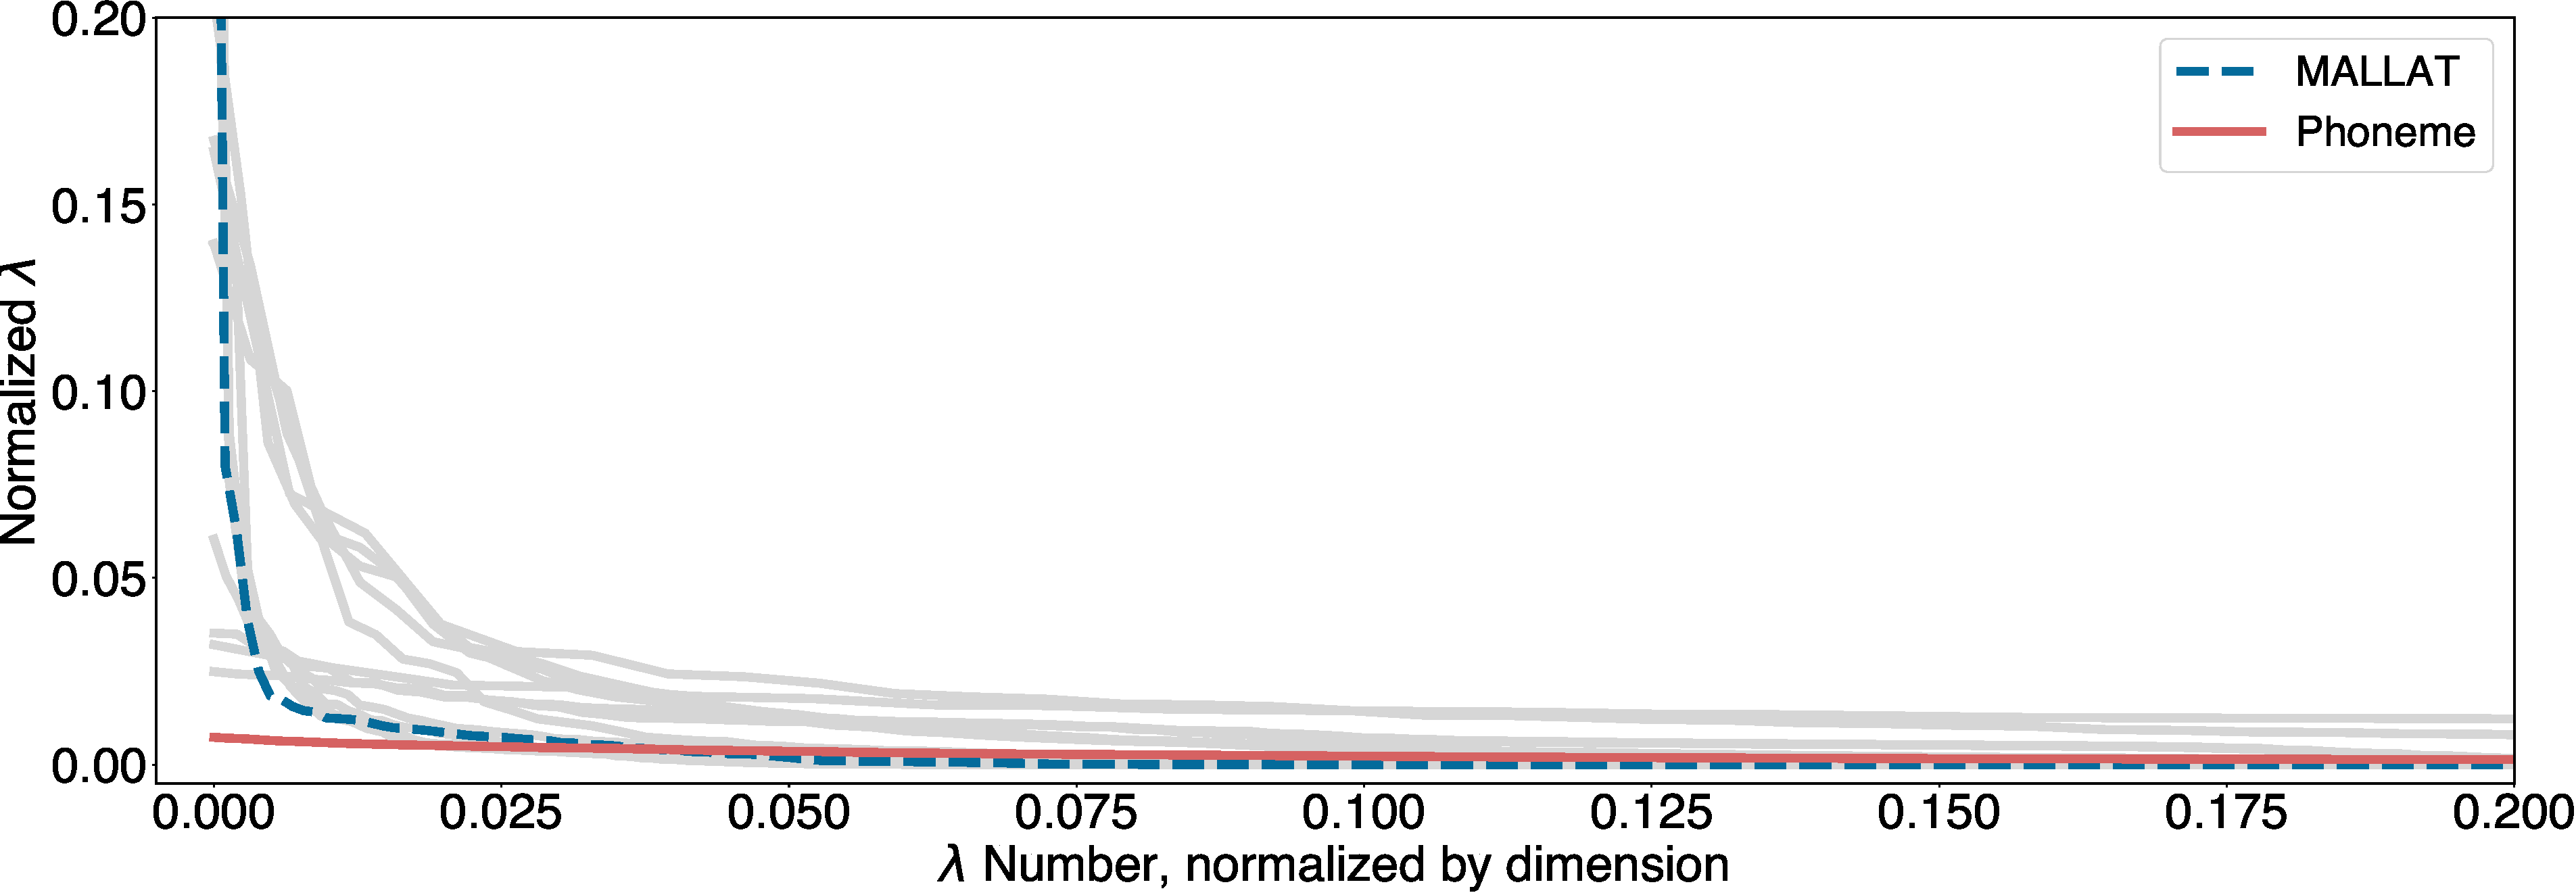
\includegraphics[width=\linewidth]{figs/spectrum-rev.pdf}
%\caption[]{Spectrum of UCR data highlighting MALLAT (performs well) and Phoneme (performs poorly).}
%\label{fig:spectrum}
%\end{figure}

%DROP can be extended to repeated-query scenarios that occur in a streaming context, where users wish to query incoming data against historical data.
%For instance, time series for similarity search are often generated as via systems that continuously monitor and obtain data from processes over a large span of time.
%Users wish to process this data as it arrives to identify anomalous or interesting behavior.
% (e.g., to identify repetitive seismic activity/earthquakes~\cite{quakes}).

Given a stationary input distribution, users can extract fixed-length sliding windows from the source and apply DROP's transformation over these segments as they arrive. 
Should the data distribution not be stationary over time, DROP can be be periodically retrained in one of two ways. 
First, DROP can use of the wide body of work in changepoint or feature drift detection~\cite{cp1, cp2} to determine when to retrain. 
Alternatively, DROP can maintain a reservoir sample of incoming data~\cite{reservoir}, tuned to the specific application, and retrain if the metric of interest no longer satisfies user-specified constraints. 
Due to DROP's default termination condition, cost-based optimization must be disabled until the metric constraint is achieved to prevent early termination.




